\FloatBarrier

\subsection*{Figures}

\begin{figure}
\centering
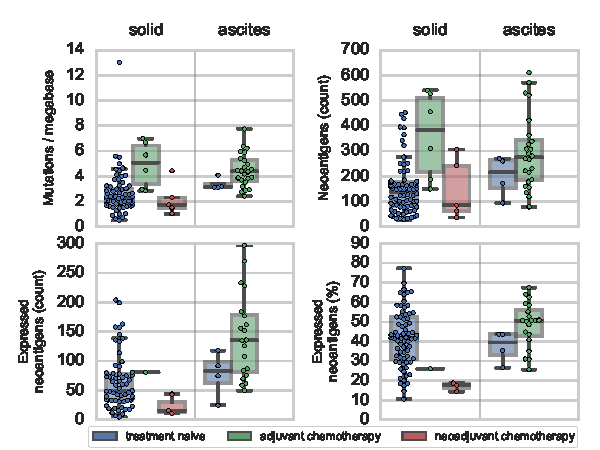
\includegraphics[scale=1.0]{figures/counts.pdf}
\caption{\textbf{Stratified comparison of mutation and neoantigen burden of chemotherapy-treated and untreated samples.} Mutations (upper left), neoantigens (upper right), and expressed neoantigens by count (lower left) and as a percent of total neoantigens (lower right) are shown for samples taken before chemotherapy (solid tumor n=75, ascites n=4), after AMCT and relapse (solid tumor n=6, ascites n=24), and after neoadjuvant chemotherapy (solid tumor n=5) (blue, green, and red, respectively). The shaded boxes indicate the interquartile region and the median line. Points indicate individual samples.}
\label{fig:counts}
\end{figure}

\begin{figure}[htbp]
\centering
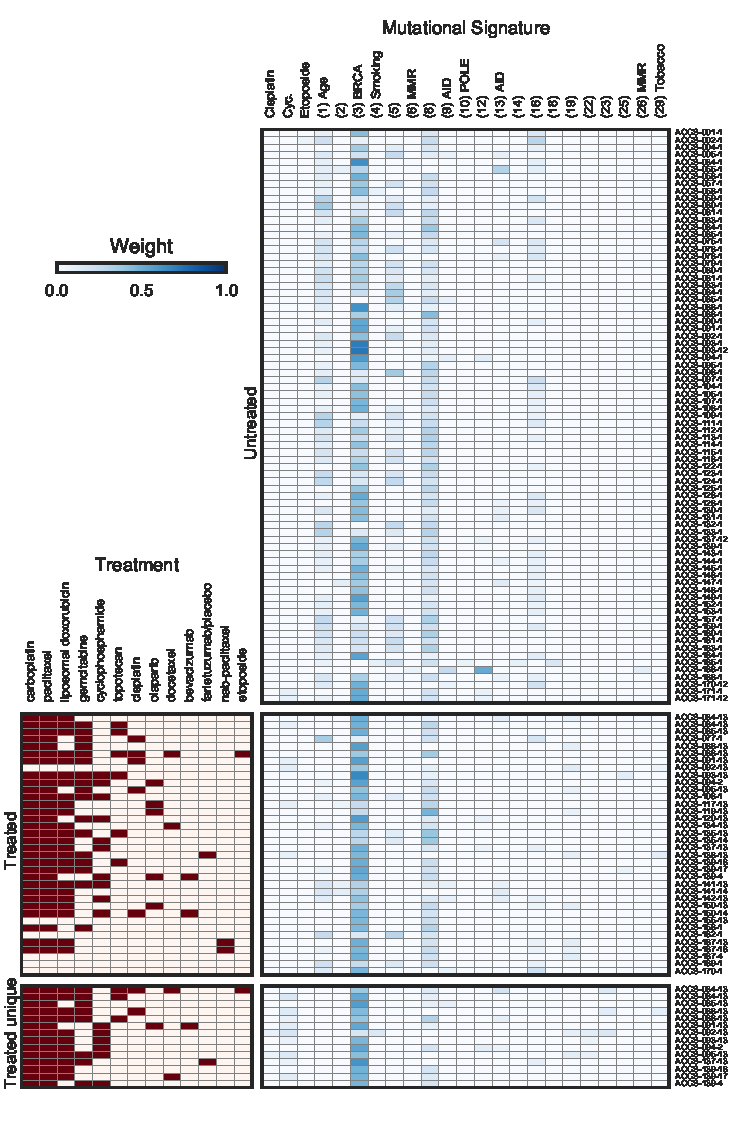
\includegraphics[scale=1.0]{figures/signatures.pdf}
\caption{\textbf{Detected mutational signatures for paired pre- and post-AMCT samples.} \textit{(Top)} Signatures detected in the pre-treatment samples. The first four signatures were extracted from reports of a \textit{G. gallus} cell line and \textit{C. Elegans} organisms after exposure to chemotherapy, and the rest are COSMIC curated signatures. COSMIC signatures numbers are shown in parentheses, and the associated mutagenic process is indicated when known. Signatures not shown were undetected in these samples. \textit{(Bottom)} Clinical treatments and detected signatures for the mutations unique to the post-treatment samples. Cases where a chemotherapy signature is detected are annotated with a (*) if the patient received the drug and a (?) otherwise.}
\label{fig:signatures}
\end{figure}

\begin{figure}[htbp]
\centering
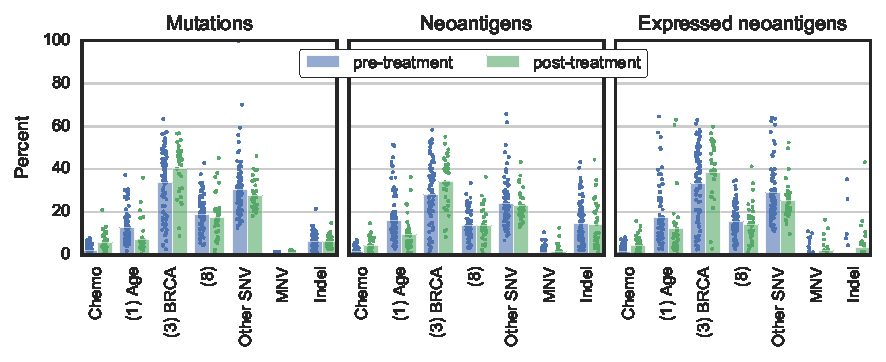
\includegraphics[scale=1.0]{figures/sources_of_mutations_and_neoantigens.pdf}
\caption{\textbf{Fraction of mutations \textit{(left)}, neoantigens \textit{(center)}, and expressed neoantigens \textit{(right)} generated by SNVs from key signatures, multinucleotide variants (MNVs), and indels.} The \textit{Chemo} category sums the contributions from the chemotherapy signatures (cisplatin, cyclophosphamide, and etoposide). COSMIC signature numbers are in parentheses. The \textit{Other SNV} category shows SNVs attributed to COSMIC signatures other than the ones shown. The bars give the mean, and the points indicate individual samples.}
\label{fig:sources}
\end{figure}

\FloatBarrier
